\documentclass[border=10pt]{standalone}

\usepackage{tikz}
\usepackage{tikzsymbols}
\usetikzlibrary{calc,patterns,shapes.geometric}

\def\centerarc[#1](#2)(#3:#4:#5){\draw[#1] ($(#2)+({#5*cos(#3)},{#5*sin(#3)})$) arc (#3:#4:#5);}

\begin{document}
	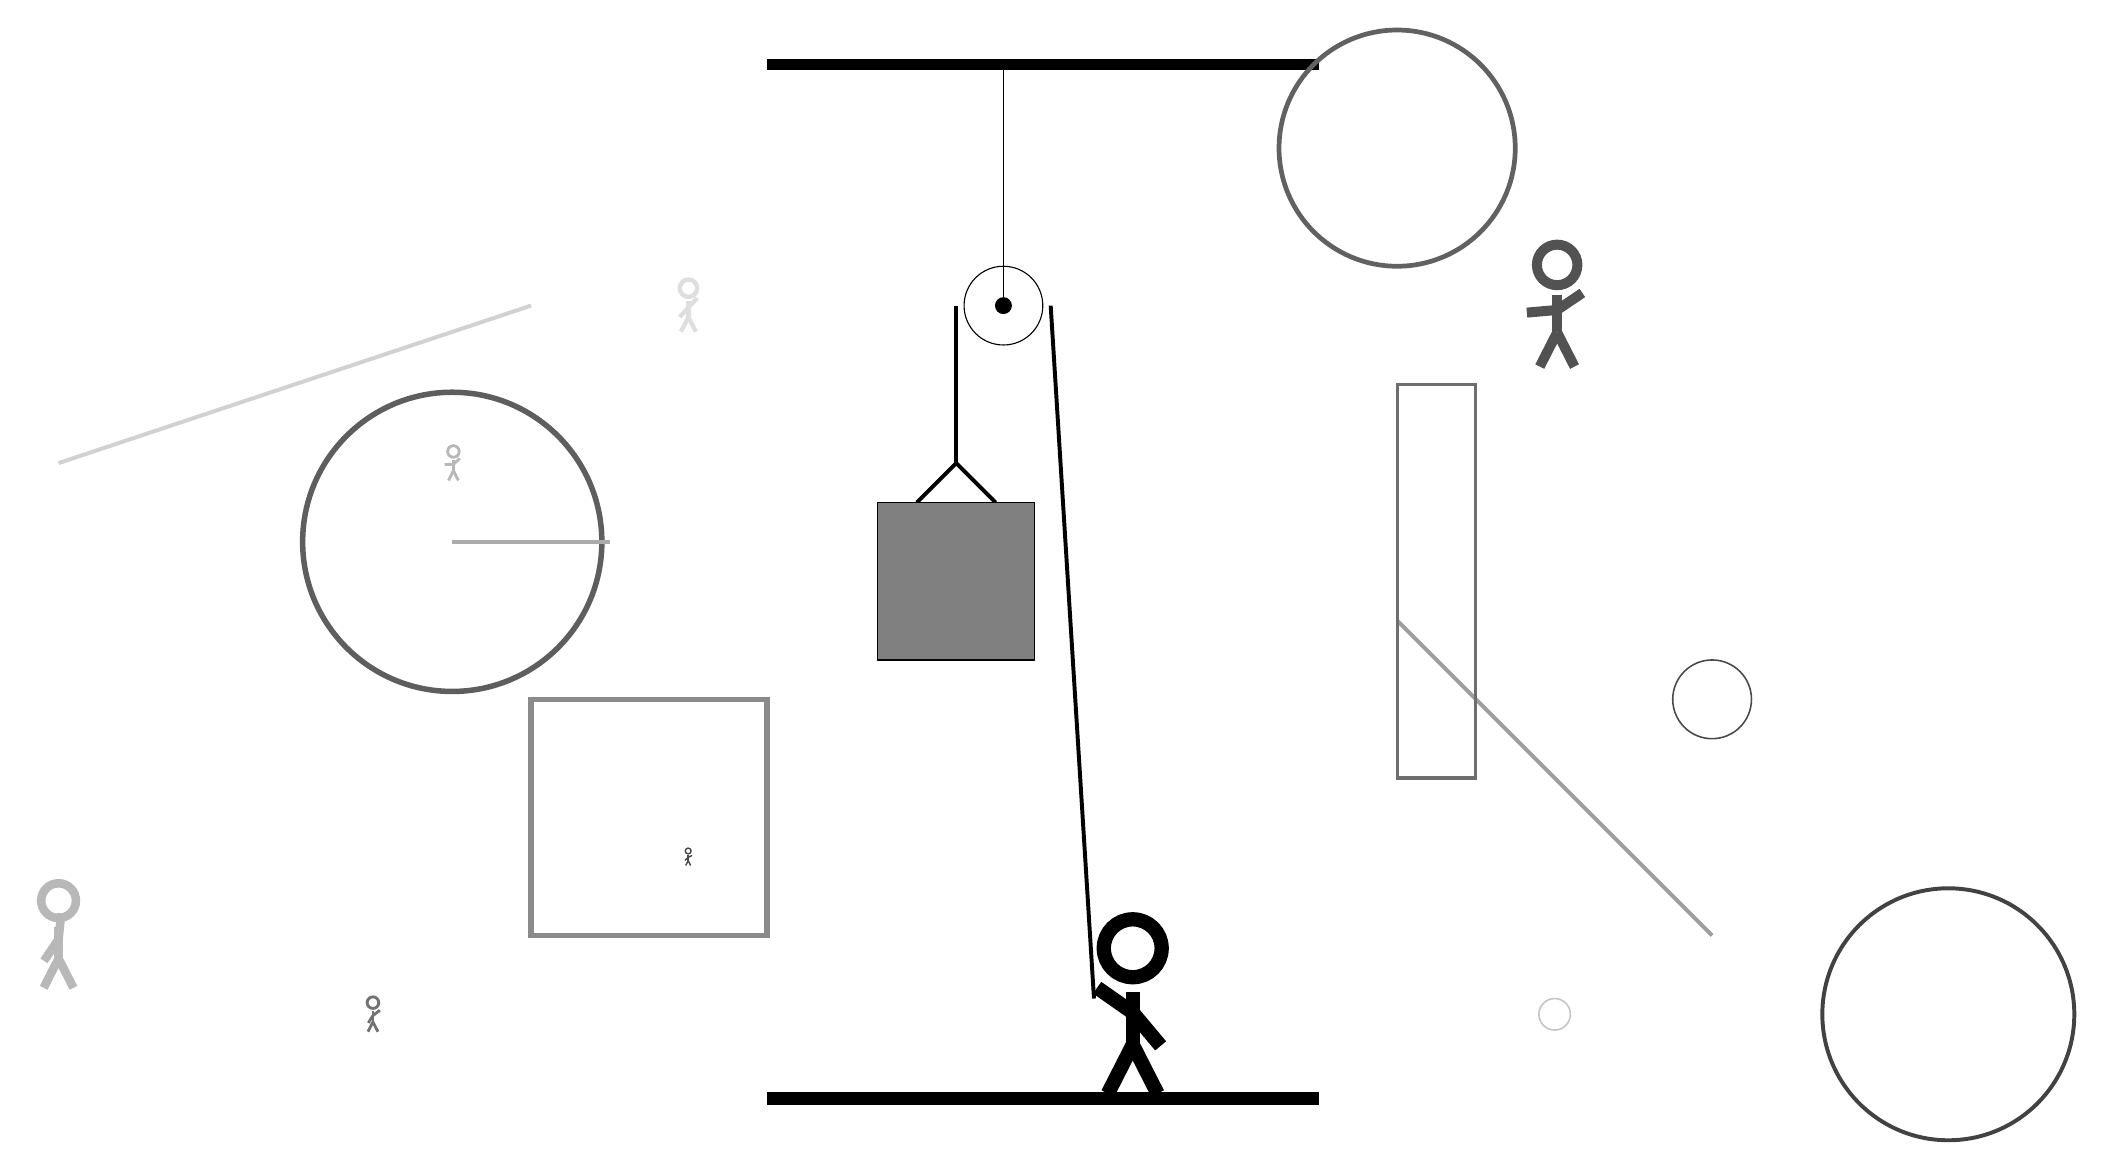
\begin{tikzpicture}
		%%%%% START %%%%%
		
		\draw[fill=black] (-2, 10) rectangle (5, 10.125);
		
		\draw (1, 7) circle (0.5);
		\draw[fill=black] (1, 7) circle (0.1);
		\draw (1, 10) -- (1, 7);
		
		\node[line width=0.7mm, color=black!55] at (-7, -2) {\Strichmaxerl[2][58][37]};
		
		\node[line width=0.7mm, color=black!71] at (-3, 0) {\Strichmaxerl[1][42][27]};
		\draw [line width=0.4mm, color=black!45](13, 5) circle (0.0);
		\draw [line width=0.5mm, color=black!74](13, -2) circle (1.6);
		\draw[line width=0.7mm, color=black!46] (-2, 2) rectangle (-5, -1);
		
		\node[line width=0.2mm, color=black!28] at (-6, 5) {\Strichmaxerl[2][1][43]};
		
		\node[line width=0.2mm, color=black!68] at (8, 7) {\Strichmaxerl[7][5][34]};
		\draw [line width=0.7mm, color=black!63](-6, 4) circle (1.9);
		\draw[line width=0.5mm, color=black!18](-5, 7) -- (-11, 5);
		\draw[line width=0.5mm, color=black!33](-6, 4) -- (-4, 4);
		\draw[line width=0.5mm, color=black!38](10, -1) -- (6, 3);
		
		\draw [line width=0.6mm, color=black!62](6, 9) circle (1.5);
		\draw [line width=0.2mm, color=black!23](8, -2) circle (0.2);
		\node[line width=0.2mm, color=black!28] at (-11, -1) {\Strichmaxerl[6][56][84]};
		\node[line width=0.4mm, color=black!13] at (-3, 7) {\Strichmaxerl[3][47][47]};
		\draw [line width=0.2mm, color=black!71](10, 2) circle (0.5);
		
		\draw[line width=0.4mm, color=black!57] (7, 1) rectangle (6, 6);
		
		\draw[line width=0.5mm] (-0.1, 4.5) -- (0.4, 5.0) -- (0.9, 4.5);
		\draw[fill=black!50] (-0.6, 4.5) rectangle (1.4, 2.5);
		
		\draw[line width=0.5mm] (0.4, 7) -- (0.4, 5.0);
		\centerarc[line width=0.5mm](1, 7)(0:180:0.6);
		\draw[line width=0.5mm](1.6, 7) -- (2.15, -1.8);
		
		\node at (2.6, -1.9) {\Strichmaxerl[10][-35][-50]};
		
		\draw[fill=black] (-2, -3) rectangle (5, -3.15);
		
		%%%%% END %%%%%
	\end{tikzpicture}
\end{document}